% Chapter Template

\chapter{Thread Coarsening} % Main chapter title

\label{Chapter3} % Change X to a consecutive number; for referencing this chapter elsewhere, use \ref{ChapterX}

\lhead{Chapter 3 \emph{Thread Coarsening}} % Change X to a consecutive number; this is for the header on each page - perhaps a shortened title

\section{What is coarsening?} \label{sec:what_is_coarsening}
Thread coarsening is an optimization technique that is often employed in GPU kernels, wherein the code that is meant to be executed by a larger number of threads gets merged into a single thread; which leads to launching fewer but more coarse-grained threads.

The nature of thread coarsening is such that it leads to a reduction in parallelism by reducing the number of threads being launched. This can, depending on the type of work being done by the kernel and the extent to which the threads are being coarsened, have a beneficial or a detrimental effect on the execution time of the kernel. To coarsen a kernel, say by a factor of 2, all instructions dependent on the thread index are duplicated, while the rest of the instructions are shared between the two coarsened instances within the kernel. These shared instructions include the CUDA API's synchronization barrier, '\_\_syncthreads()', which features quite commonly in the convolution kernels employing shared memory optimizations.

\begin{figure}[ht]
	\centering
	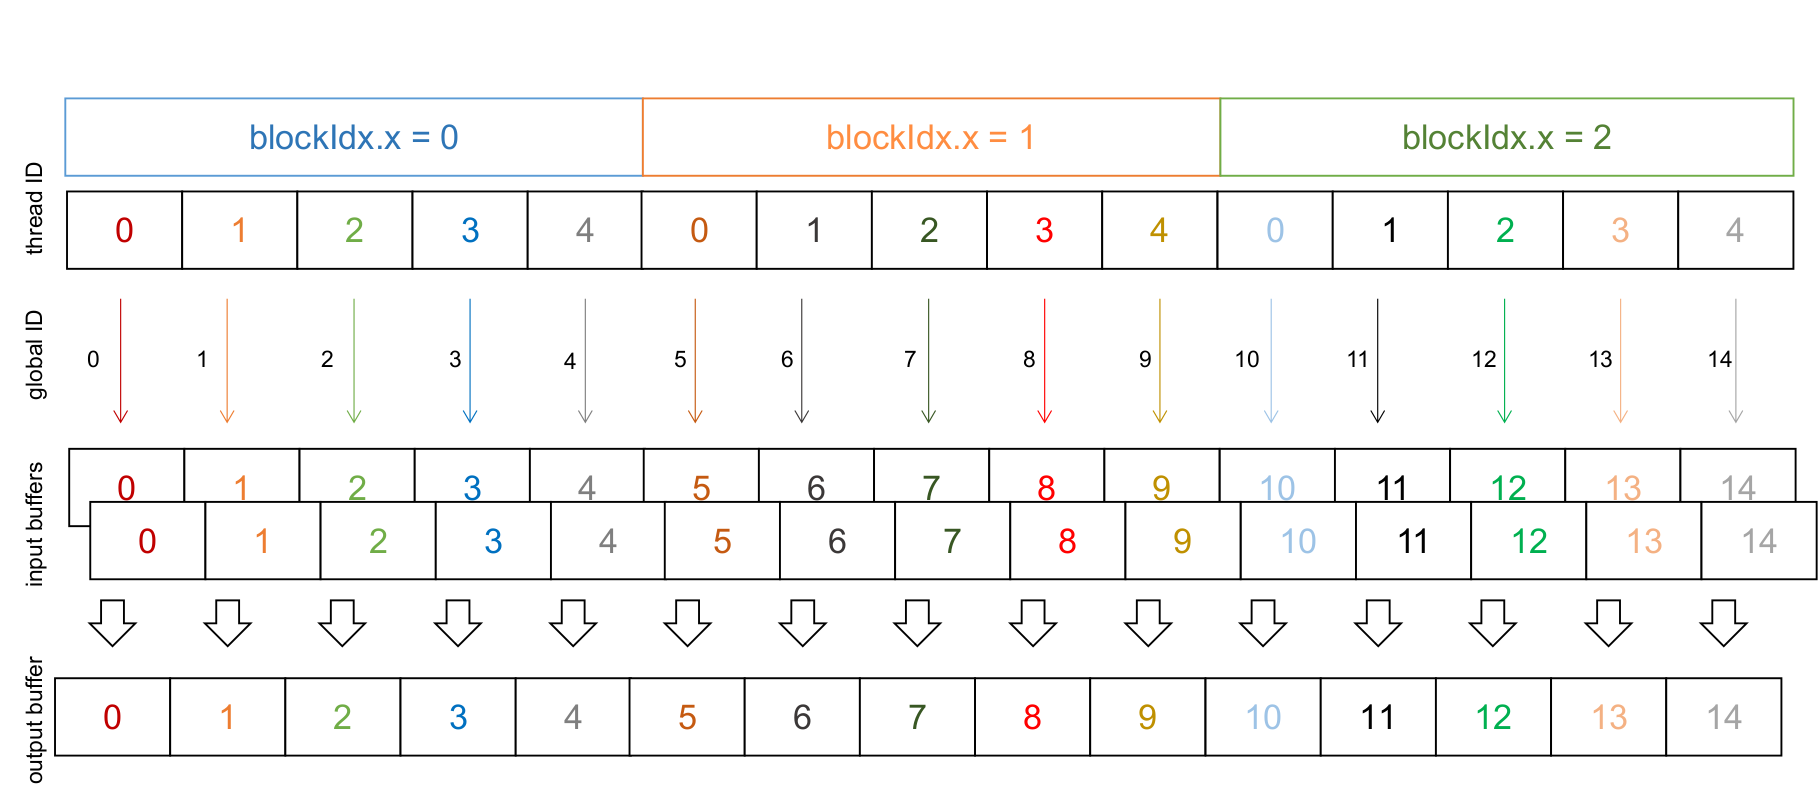
\includegraphics[scale=0.25]{Pictures/ch3/thread_allocation.png}
	\caption{\small CUDA thread mapping}
\end{figure}


\begin{figure}[ht]
	\centering
	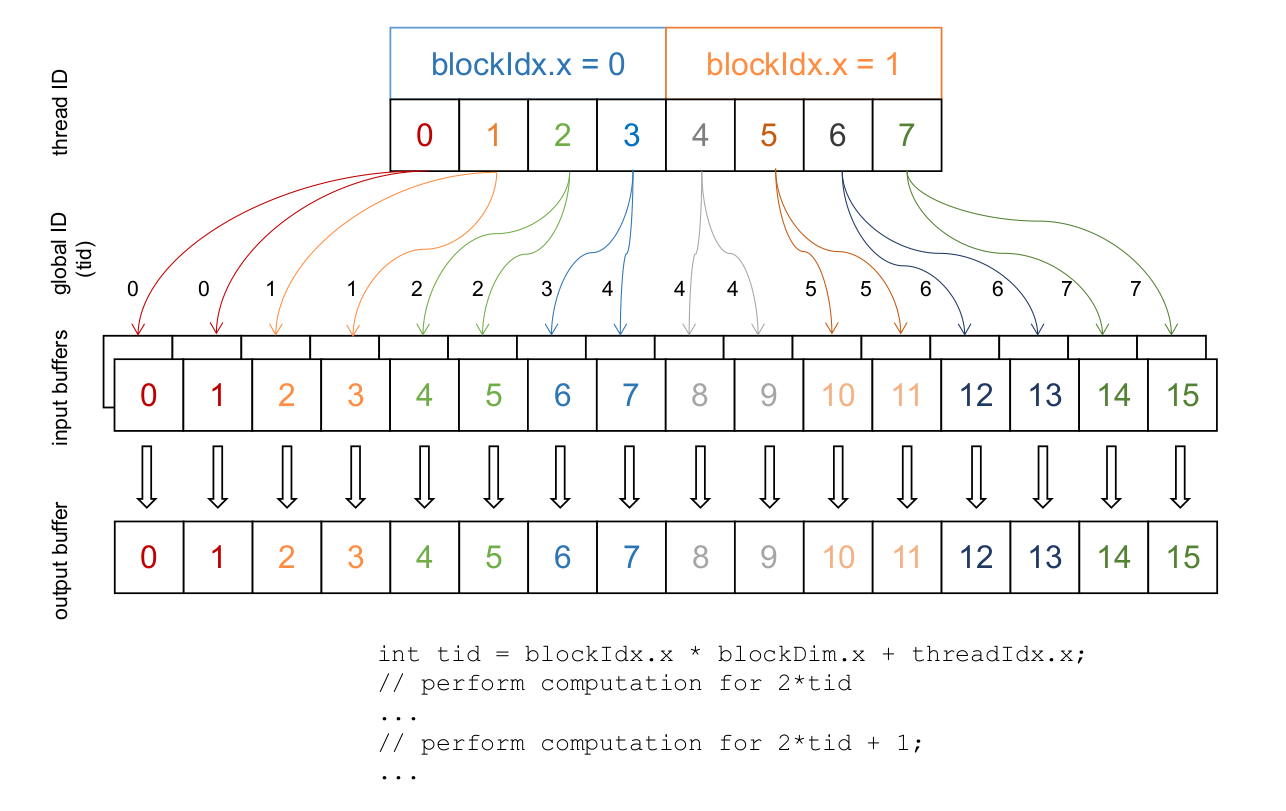
\includegraphics[scale=0.35]{Pictures/ch3/coarsen_2C2S.png}
	\caption{\small CUDA thread coarsening for C = 2, S = 2}
\end{figure}

\begin{figure}[ht]
	\centering
	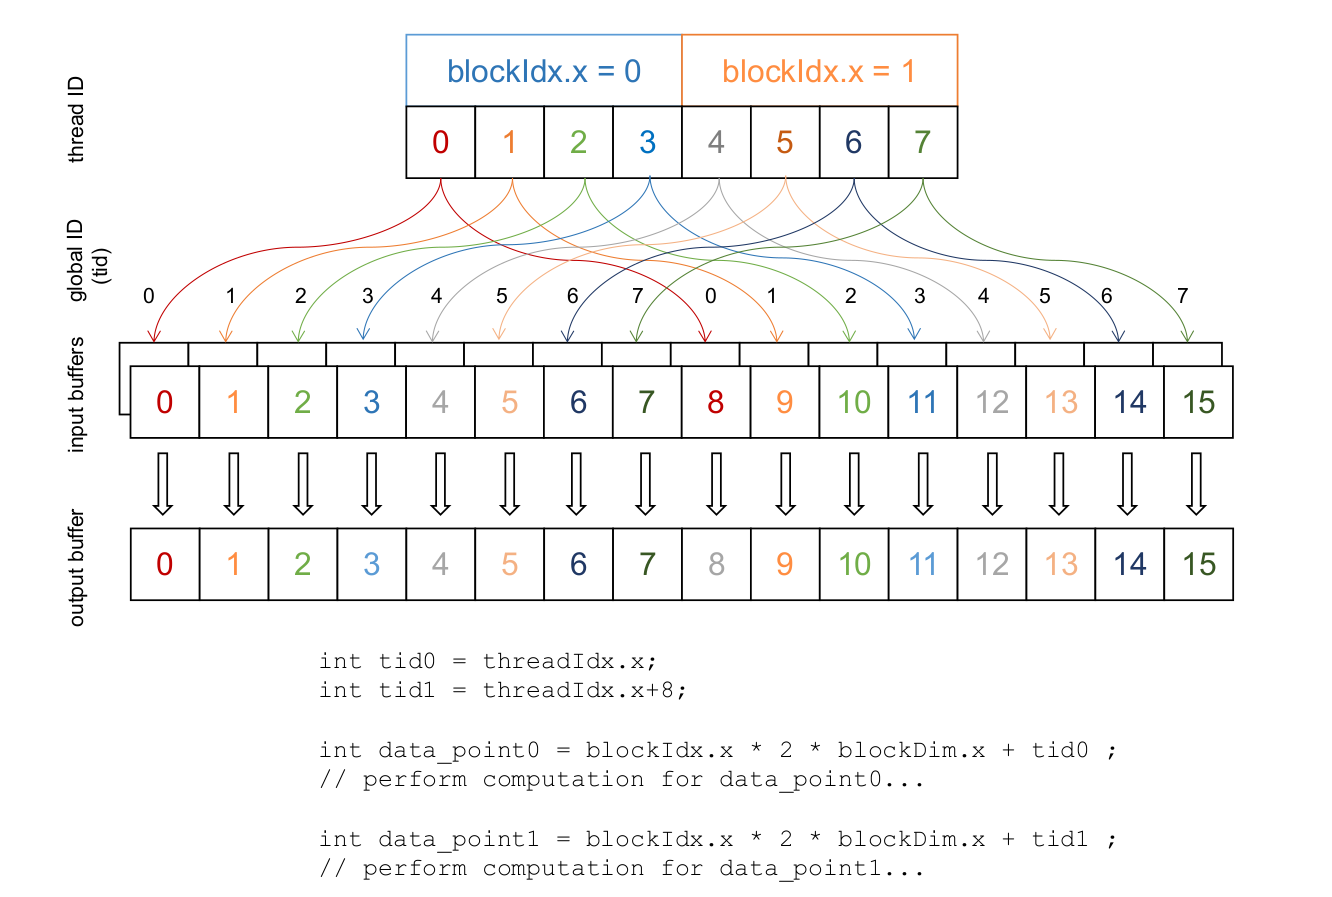
\includegraphics[scale=0.35]{Pictures/ch3/coarsen_2C8S.png}
	\caption{\small CUDA thread coarsening for C = 2, S = 8}
\end{figure}


\begin{figure}[ht]
	\centering
	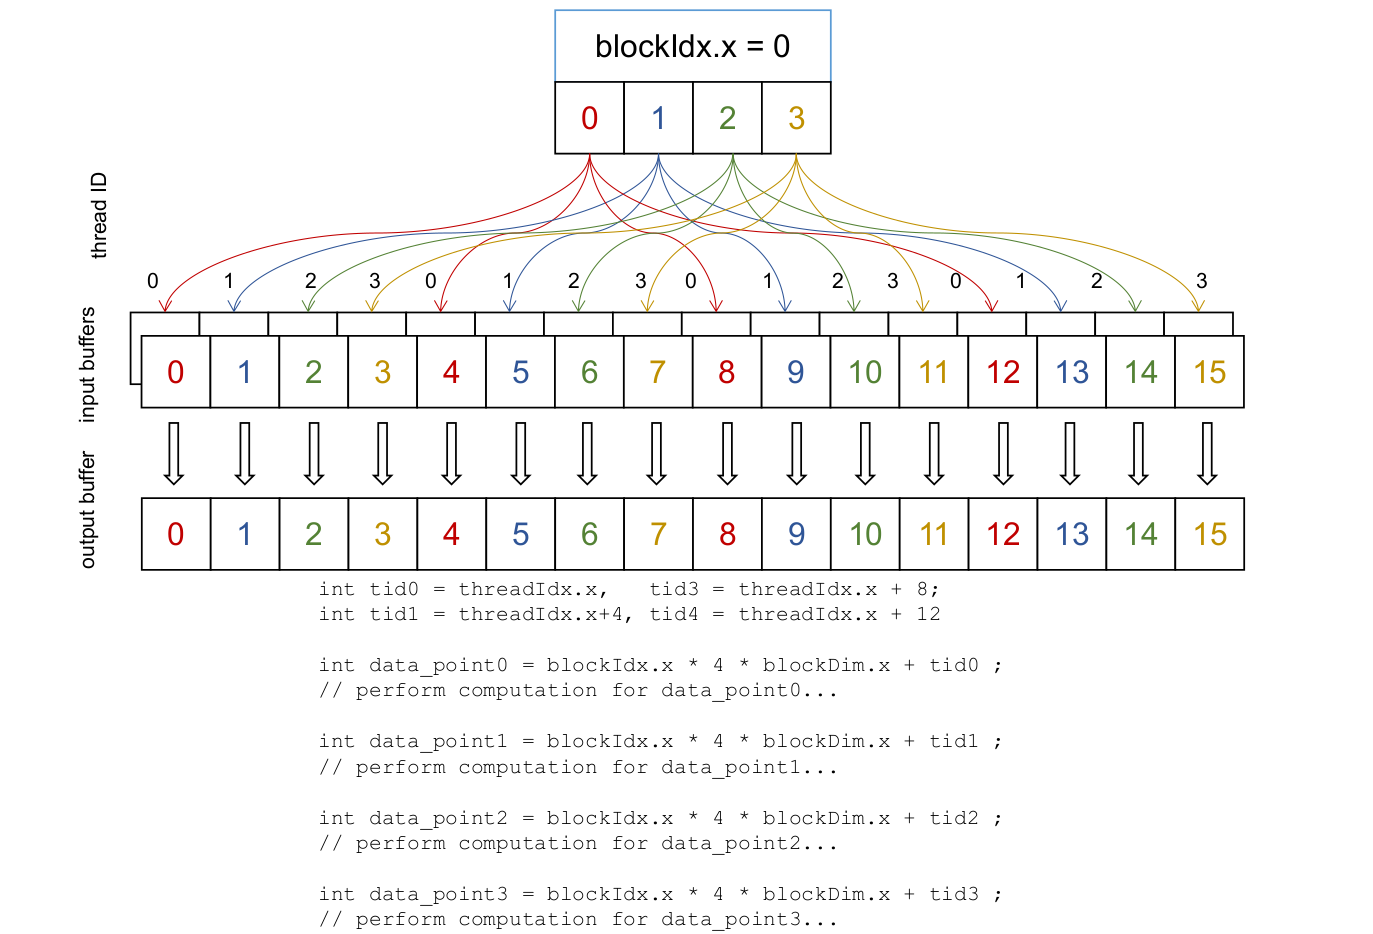
\includegraphics[scale=0.35]{Pictures/ch3/coarsen_4C4S.png}
	\caption{\small CUDA thread coarsening for C = 4, S = 4}
\end{figure}

\section{Effects of coarsening} \label{sec:effect_of_coarsening}

Thread coarsening, by the virtue of being an optimization technique, allows programmers to maximize GPU utilization, and reduce the execution-time of kernels. However, as mentioned in the preceding section, this can, depending on several factors, also lead to a decrease in the parallelism, and consequently, the performance of the kernel. In this work, I have tried to better understand and provide a theoretical justification to the performance changes we see in the convolution kernels when coarsened to different extents.

To understand how coarsening affects kernels and try and predict whether coarsening might be helpful for a given convolution kernel with fixed hyper-parameters, we first need to understand the broad changes that are introduced when a kernel is coarsened.

The biggest, and perhaps the most evident change brought by coarsening is the reduction in the number of threads that are launched to finish the execution of the code. As each thread now performs the work that was previously done by multiple threads, the number of threads launched reduces by a factor of the number of threads whose work is fused into one, more commonly known as the coarsening factor. Thus, for a convolution kernel coarsened by a factor of 8, if the original kernel was launched with 256 threads; the coarsened kernel will be launched with only 32 threads.

This reduction in the size of thread block being launched for a kernel leads to an improvement in the kernel execution time in primarily three ways:

i. smaller thread blocks lead to a greater number of concurrent blocks being scheduled on the same SM, which reduces the number of batches that need to be executed to complete the computation. This leads to an improvement by cutting down on the overhead that accompanies scheduling and executing thread blocks on the SM.

ii. fewer number of threads launched leads to a lesser number of barrier calls made, taken over the entire execution of the program

iii. greater number of instructions per thread leads to better exploitation of hardware instruction-level parallelism.

One would expect these advantages to scale with the coarsening factor, which they do to some extent. As the level of coarsening increases, we eventually reach a point where the reduction in parallelism due to the extensive coarsening can no longer be compensated for by the advantages mentioned above. From this point on, any further attempts at coarsening the kernel only lead to a decrease in the observed performance.  

In addition to this reduction in parallelism, the coarsened threads are also more resource-hungry. As the work being done by the threads in a coarsened kernel is more, it raises the thread block's resource requirements, such as the number of registers and shared memory needed, which in turn lead to a reduced occupancy. Thus, when it comes to thread coarsening, there is a very clear performance tradeoff at play, and the problem of identifying the optimal coarsening factor (or deciding no coarsening is beneficial) for a given kernel is still a non-trivial problem.

In the next section, we will compare the performance of a convolution kernel against itself when coarsened to different extents, and try to provide some theoretical justification to the results observed.

\section{Results \& Observations} \label{sec:predict_coarsening}

The first part of the project done in this semester deals with the implementation of a single parameterized pass that can automatically coarsen convolution kernels with a user-defined value of coarsening factor and stride, and generate the CUDA code for the same. This was implemented using a macro processor known called PyExpander, which allows Python code to be embedded in text files. Coarsening by definition involves repetition of instructions which are dependent on thread indices. Thus, for a given convolution kernel, the script uses loops in the text file to replicate the relevant statements.

\begin{figure}[ht]
	\centering
	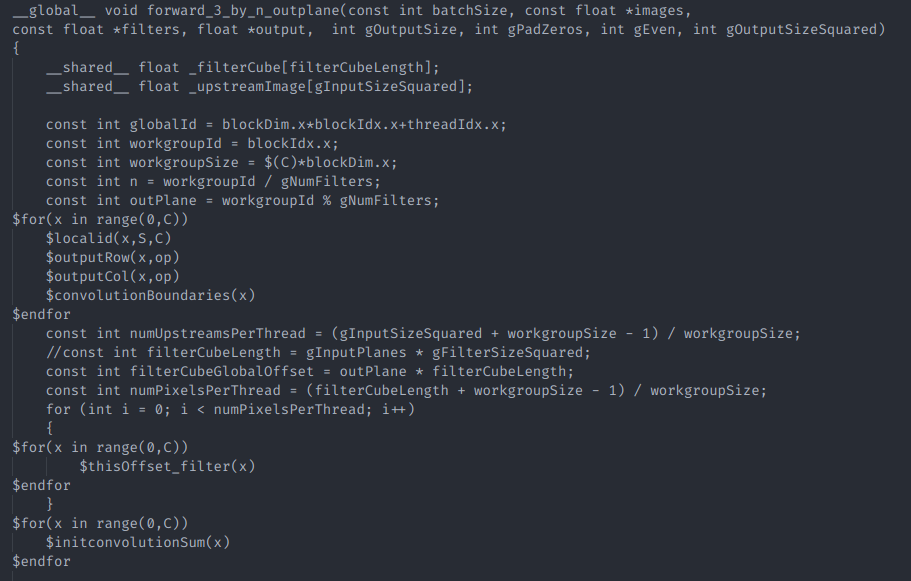
\includegraphics[scale=0.45]{Pictures/ch3/script.png}
	\caption{\small PyExpander script for generating coarsened kernels}
\end{figure}

Such a script allows generation of coarsened kernels with custom coarsening factors, which is vital in the development of the CUDA scheduler that determines optimal coarsening factors depending on the available hardware resources at any moment. This serves an important purpose of not having to generate the coarsened kernels for different values of C prior to kernel launch, and more importantly, provides the system with the flexibility to determine an appropriate coarsening factor without any constraints on the values allowed.

\begin{figure}[ht]
	\centering
	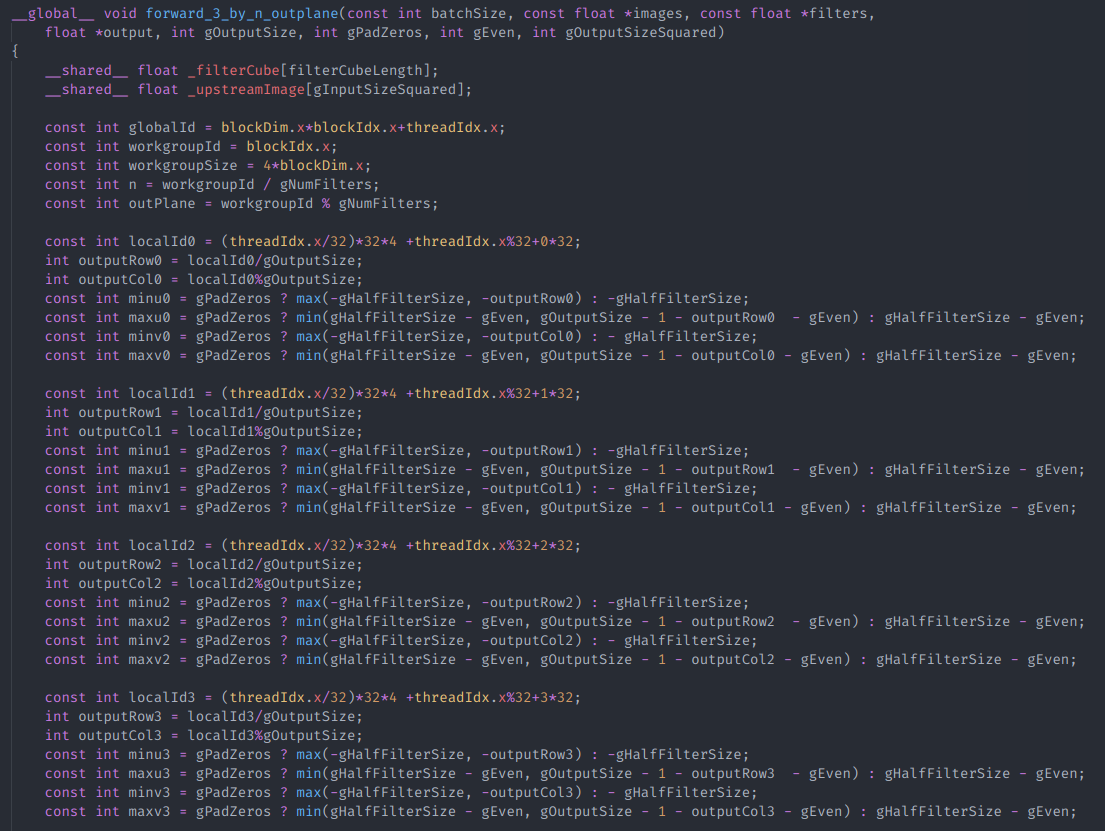
\includegraphics[scale=0.4]{Pictures/ch3/code coarsened.png}
	\caption{\small Coarsened convolution kernel for C=4}
\end{figure}


As mentioned in the preceding section, the effects of thread coarsening are not uniform and instead depend on the kernel being coarsened. For our specific problem, focused on CNN pipelines and attempting to coarsen the convolution kernels, the difference in kernels arise from the changes in hyper-parameters such as the size of the input, number of channels in the input input, number of filters, etc. Simply modifying these hyper-parameters without changing any other part of the kernel code can significantly alter the behavior changes we see due to coarsening in the kernel. To study the effects of coarsening and try to justify them, we will first limit ourselves to a specific set of hyper-parameters values and observe the results when this kernel is coarsened using different coarsening factors.


The kernel we are going to analyse is a 3D convolution kernel, which computes performs convolution of multiple images in a batch with a given filter in a single pass. The kernel is optimized by making use of shared memory for faster repeated read operations while performing the convolution. The hyper-parameters for this experiment are as follows:

\begin{itemize}
\item batch size: 1024
\item size of single channel in input image: 31 x 31
\item number of channels in input image: 5
\item size of single channel in input filter: 3 x 3
\item number of filters: 2
\end{itemize}

The speedups for this kernel's coarsened variants are given in table 3.1, and visualised in fig 3.7

% \begin{table}[ht]
%     \centering
    
%     \begin{tabular}{ |p{5cm}|p{5cm}|  }
%          \hline
%          Coarsening factor & Execution time (in ms) \\
%          \hline
%          1 (Uncoarsened)    & 1.66\\
%          2                  & 1.09\\
%          4                  & 0.91\\
%          8                  & 1.08\\
%          16                 & 1.58\\
%          32                 & 5.73\\
%          \hline
%     \end{tabular}
%     \caption{\small Execution times for different coarsening factors}
%     \label{tab:execution_time_good_coarsen}
% \end{table}

\begin{figure}[ht]
	\centering
	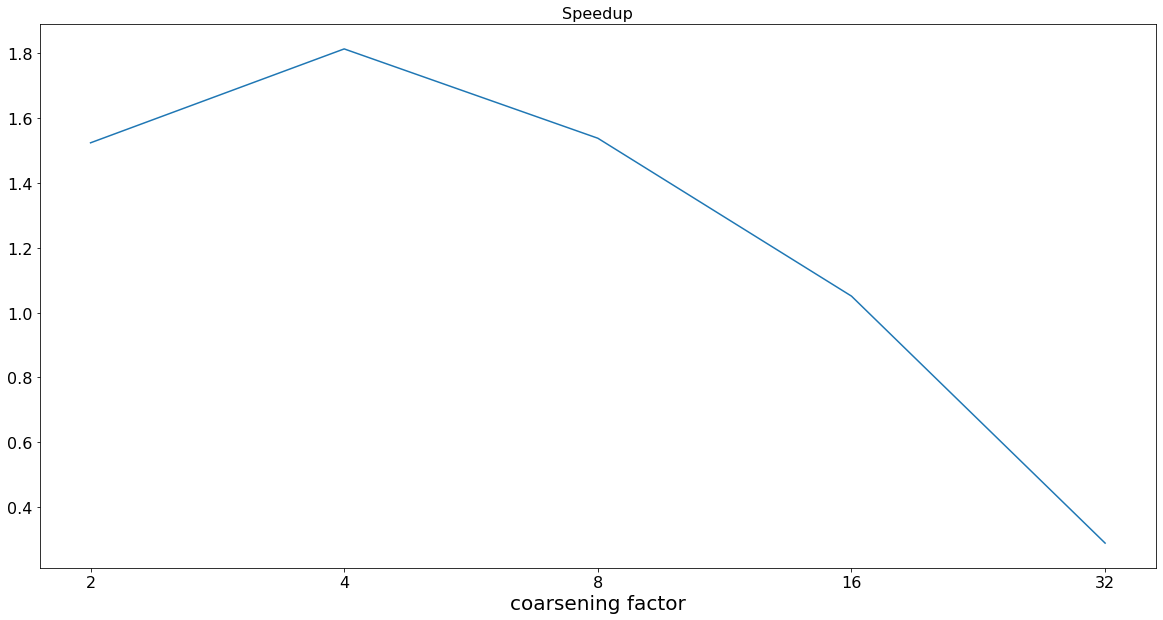
\includegraphics[scale=0.30]{Pictures/plots/good_improvement_coarsening/speedup.png}
	\caption{\small Speedup for differently coarsened kernels - Case I}
\end{figure}

A cursory look at the data seems to match the hypothesis we had established so far of decreased execution time with increase in the coarsening factor till a limit (in this example, that limit is 4), following which the performance starts degrading rapidly.

In order to justify this behavior, let us also look at the block size in each of these cases from table 3.1.

% \begin{table}[ht]
%     \centering
    
%     \begin{tabular}{ |p{5cm}|p{5cm}|  }
%          \hline
%          Coarsening factor & Thread block size \\
%          \hline
%          1 (Uncoarsened)    & 841\\
%          2                  & 448\\
%          4                  & 224\\
%          8                  & 128\\
%          16                 & 64\\
%          32                 & 32\\
%          \hline
%     \end{tabular}
%     \caption{\small Size of thread blocks for different coarsening factors}
%     \label{tab:block_size_good_coarsen}
% \end{table}

The maximum number of resident threads allowed on an SM at any given time, for the hardware on which these experiments were conducted, is 2048. Therefore, following the size of thread blocks as given in table 3.1, we see that the reduction in the size of thread block allows for more blocks to be scheduled and executed concurrently on the SMs. This reduces the number of batches for which execution needs to be performed, as more data is now being processed per batch, which in turn leads to a decrease in the execution time due to the overhead associated with scheduling and execution of batches in the SM. However, as table 3.1 also makes very evident, this justification does not extend beyond a coarsening factor of 4, at which point onward, even with a decrease in the size of the thread block, the execution time starts to rise.

To understand this behavior, we need to introduce another metric in our analysis, the register pressure. As the kernel is coarsened, and number of threads reduces, each individual thread performs more instructions, and in turn requires greater number of registers to execute. The number of registers required per thread to execute the kernel is known as the register pressure, or the registers per thread. For the kernel under consideration, the register pressure varies as seen in figure 3.8.

\begin{figure}[ht]
	\centering
	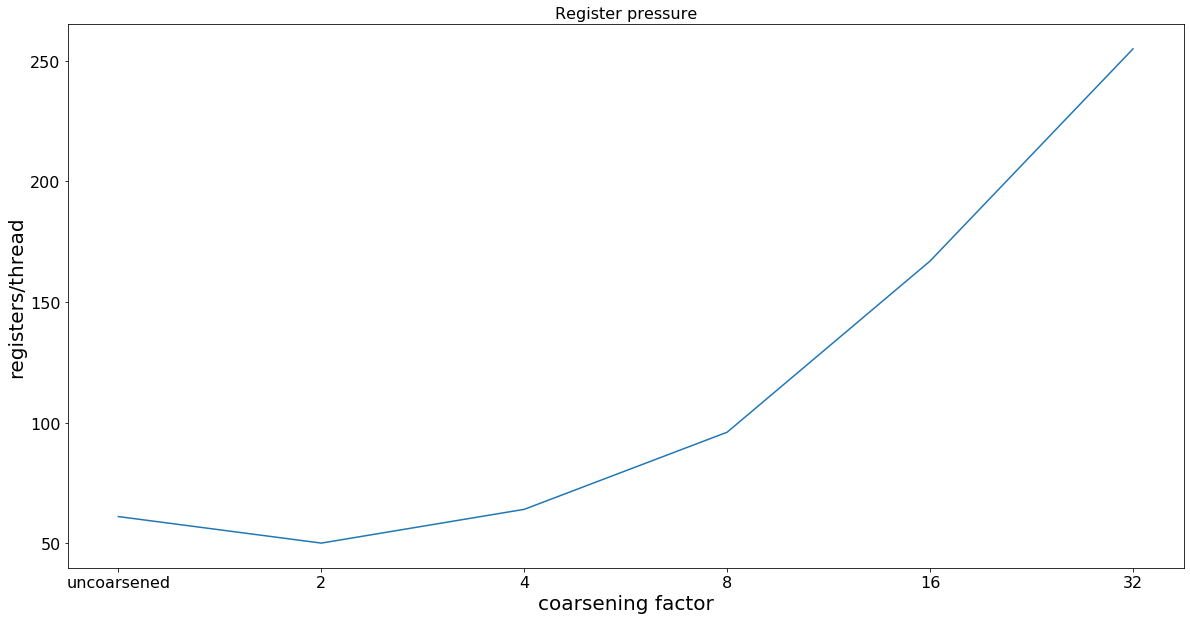
\includegraphics[scale=0.30]{Pictures/plots/good_improvement_coarsening/register pressure.png}
	\caption{\small Register for differently coarsened kernels - Case I}
\end{figure}

% \begin{table}[ht]
%     \centering
    
%     \begin{tabular}{ |p{5cm}|p{7cm}|  }
%          \hline
%          Coarsening factor & Register pressure (registers/thread) \\
%          \hline
%          1 (Uncoarsened)    & 61\\
%          2                  & 50\\
%          4                  & 64\\
%          8                  & 96\\
%          16                 & 167\\
%          32                 & 255\\
%          \hline
%     \end{tabular}
%     \caption{\small Register pressure for different coarsening factors}
%     \label{tab:block_size_good_coarsen}
% \end{table}

Apart from the anomaly seen when going from an uncoarsened kernel to a coarsening factor of 2, the register pressure shows a regular trend with the decrease in the number of threads launched. With increase in the coarsening factor, each thread is responsible for carrying out more instructions, which is seen as an increase in the register pressure. For coarsening factor of 32, the register pressure exceeds the maximum hardware limit of 255, and the remaining registers are accessed from the global memory, a phenomenon known as register spilling.

An increased register pressure implies a greater resource demand for each warp scheduled on the SM. As the resources available on any SM are limited, this in turn leads to another potential parameter which could act as a bottleneck in terms of scheduling and execution of thread blocks. For the hardware used for this experiment, the number of registers present in an SM is 65,536. From table 3.1, for kernel with coarsening factor of 4, this would correspond to a maximum of 65,536/(32*64) = 32 warps concurrently scheduled warps in an SM. On the other hand, for coarsening factor of 8 and register pressure of 96, this number reduces to 65,536/(96*32), or just 21 active warps per SM. The theoretical (and the achieved) occupancy, therefore, are determined not just by one but multiple factors as demonstrated in this section. Apart from register pressure, other parameters such as shared memory per block can also act as a potential bottleneck. However, in our experiment, the amount of static shared memory per block does not change with the coarsening factor and therefore, can be ignored for purposes of evaluating change in the performance levels with different extents of coarsening. 

The results presented above can be in a summarised in a table as follows. In addition to the execution time and register pressure, we have also provided the theoretical and achieved occupancy for each of the cases, along with the \% utilization of the SM (on average) for each case.


\begin{table}[ht]
    \centering
    
    \begin{tabular}{ |p{2cm}|p{1.5cm}|p{1.5cm}|p{2cm}|p{2cm}|p{2cm}|p{2cm}|  }
         \hline
         Coarsening factor & Block size & Register pressure & Theoretical Occupancy & Achieved Occupancy & SM Utilization & Execution time (in ms) \\
         \hline
         
         1    & 841 & 61 & 84.38 & 83.32 & 43.44 & 1.66\\
         2                  & 448 & 50 & 87.5 & 85.96 &62.26 &  1.09\\
         4                  & 224 & 64 & 87.5 & 86 & 69.98 & 0.91\\
         8                  & 128 & 96 & 62.5 & 61.42 & 63.91 & 1.08\\
         16                 & 64 & 167 & 37.5 & 34.26 & 41.51 & 1.58\\
         32                 & 32 & 255 & 25 & 24.13 & 23.99 & 5.73\\
         \hline
    \end{tabular}
    \caption{\small Comparison of occupancy and execution time variation with coarsening factor - Case I}
    \label{tab:block_size_good_coarsen}
\end{table}



\begin{figure}[ht]
	\centering
	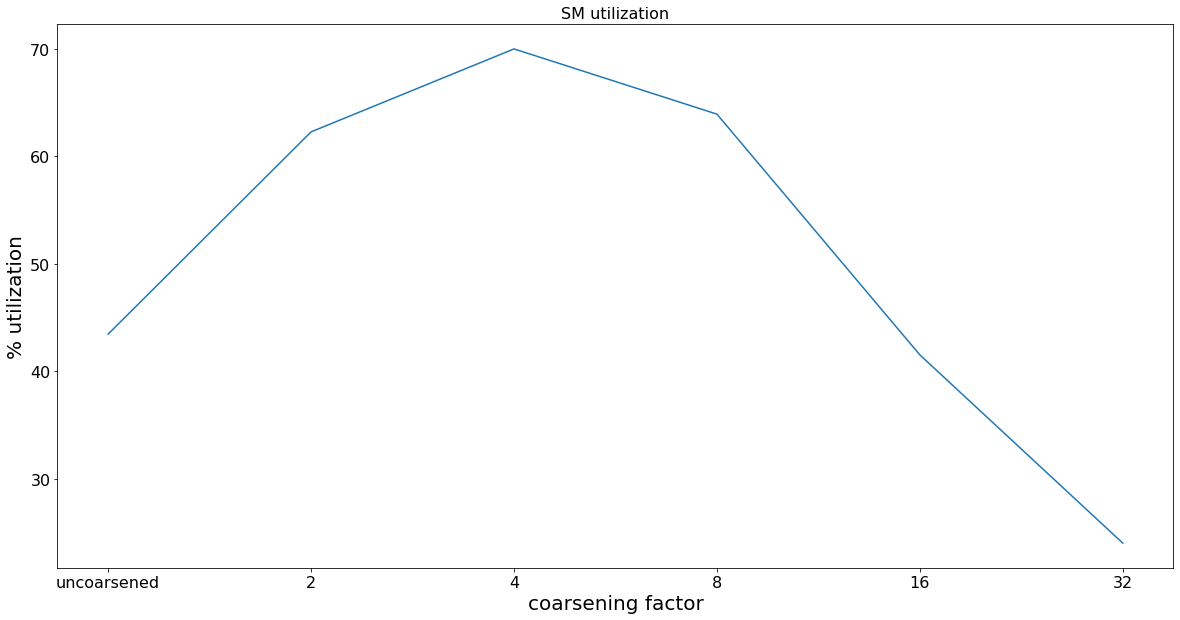
\includegraphics[scale=0.30]{Pictures/plots/good_improvement_coarsening/sm util.png}
	\caption{\small SM utilization for differently coarsened kernels - Case I}
\end{figure}

\begin{figure}[ht]
	\centering
	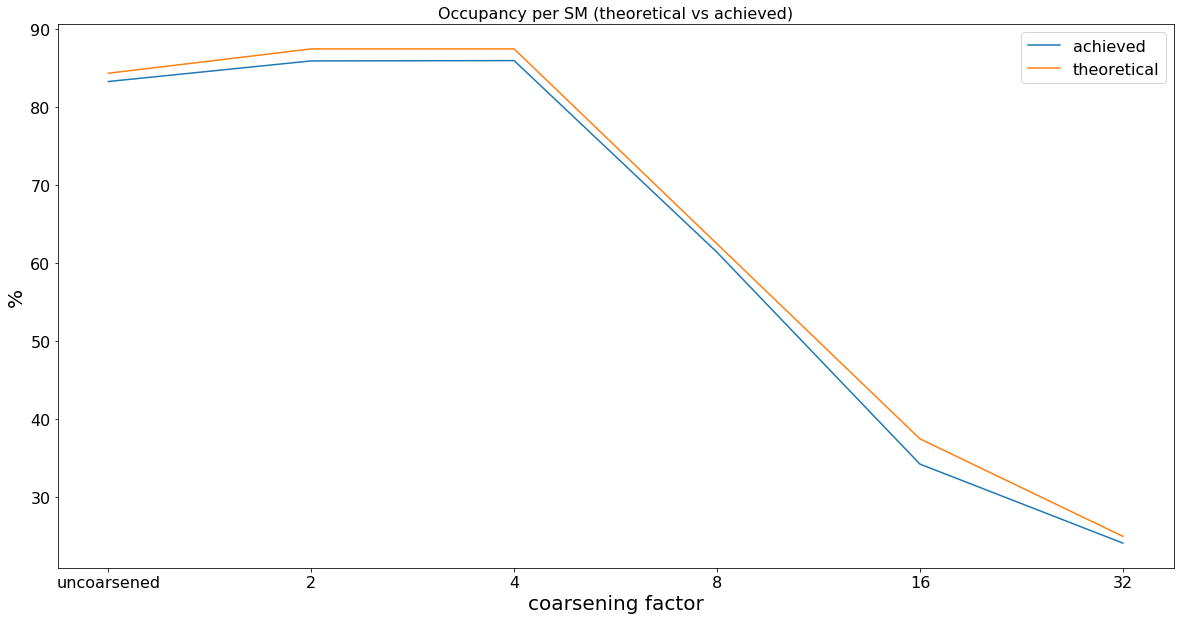
\includegraphics[scale=0.30]{Pictures/plots/good_improvement_coarsening/occupancy.png}
	\caption{\small Occupancy for differently coarsened kernels - Case I}
\end{figure}


Let us now consider the same convolution kernel with a different set of hyper-parameters where coarsening leads to a different trend in the variation of performance:


\begin{itemize}
\item batch size: 1024
\item size of single channel in input image: 45 x 45
\item number of channels in input image: 5
\item size of single channel in input filter: 15 x 15
\item number of filters: 2
\end{itemize}

The execution time for this kernel and the different coarsened variants is given below:

\begin{figure}[ht]
	\centering
	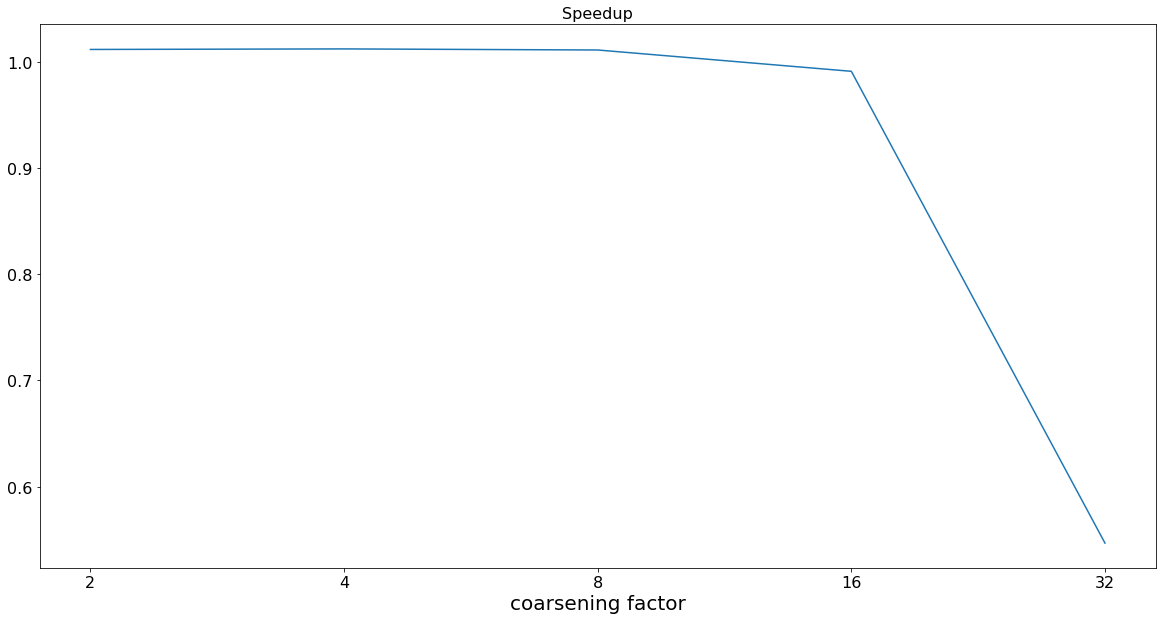
\includegraphics[scale=0.30]{Pictures/plots/poor_improvement/speedup.png}
	\caption{\small Speedup for differently coarsened kernels - Case II}
\end{figure}

In contrast to figure 3.7, we see that the speedup for this kernel isn't significant at all. While smaller coarsening factors ( less than 16 ) barely show any improvement in performance in terms of the execution time, further coarsening leads to a sharp degradation instead.

In order to understand this seemingly strange behavior, let us first observe the trend in occupancy because of the coarsening.

\begin{figure}[ht]
	\centering
	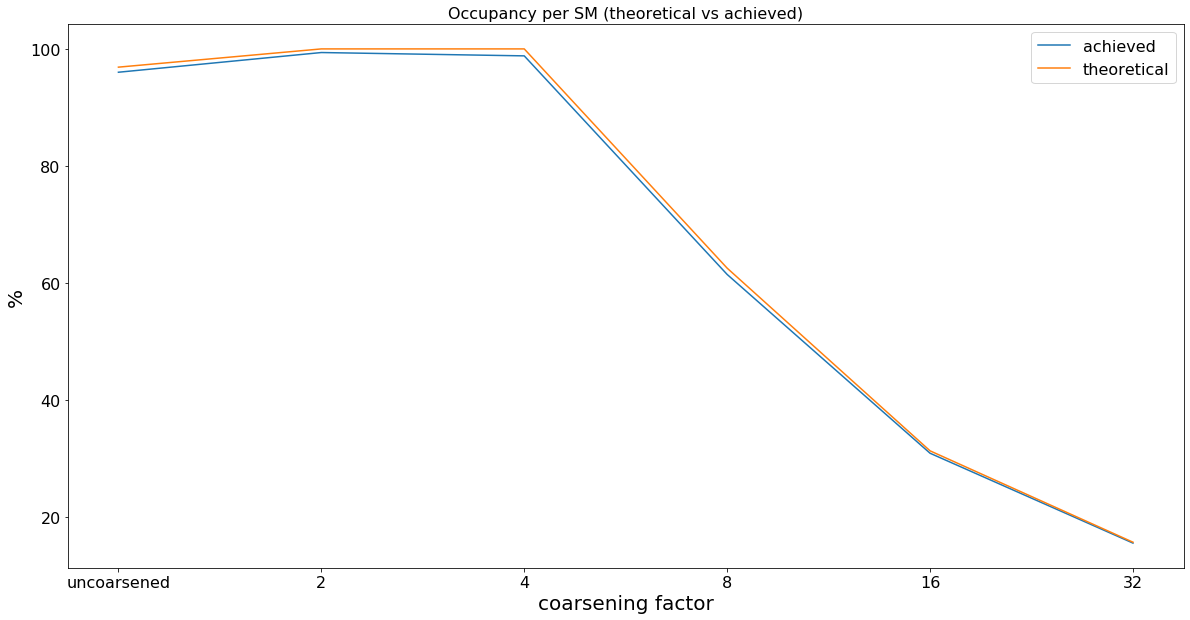
\includegraphics[scale=0.30]{Pictures/plots/poor_improvement/occupancy both.png}
	\caption{\small Occupancy for differently coarsened kernels - Case II}
\end{figure}

As one would expect after looking at the speedups, the occupancy does not change in any significant manner for small coarsening factors. However, for large coarsening factors, it shows a sharp decline and quickly falls off to sub-optimal levels.

Similar to the previous case, let us again try and see if the register pressure can tell us something about the observations for this case from figure 3.13.

\begin{figure}[ht]
	\centering
	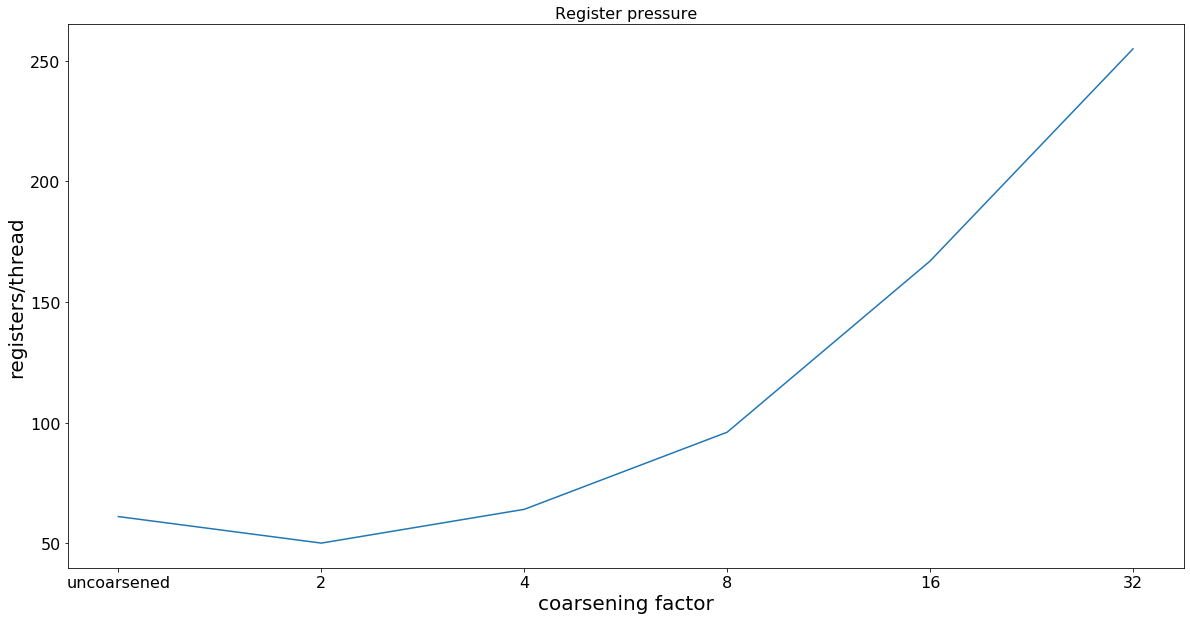
\includegraphics[scale=0.30]{Pictures/plots/poor_improvement/reg pressure.png}
	\caption{\small Register pressures for differently coarsened kernels - Case II}
\end{figure}

Notice that this trend is identical to what we saw in the previous case (fig. 3.8)! This reinforces our previous conclusion that occupancy (and the execution time observed) is not a uni-variate function (of register pressure) but depends on a lot of factors instead.

\begin{table}[ht]
    \centering
    
    \begin{tabular}{ |p{2cm}|p{1.5cm}|p{1.5cm}|p{2cm}|p{2cm}|p{2cm}|p{2cm}|  }
         \hline
         Coarsening factor & Block size & Register pressure & Theoretical Occupancy & Achieved Occupancy & SM Utilization & Execution time (in ms) \\
         \hline
         
         1                  & 992 & 61 & 96.88 & 96.01 & 64.63 & 19.97\\
         2                  & 512 & 50 & 100 & 99.31 & 68.09 & 19.73\\
         4                  & 256 & 64 & 100 & 98.81 & 68.09 & 19.72\\
         8                  & 128 & 96 & 62.5 & 61.42 & 68.02 & 19.74\\
         16                 & 64 & 167 & 31.25 & 30.84 & 66.56 & 20.14\\
         32                 & 32 & 255 & 15.62 & 15.47 & 37.55 & 36.53\\
         \hline
    \end{tabular}
    \caption{\small Comparison of occupancy and execution time variation with coarsening factor - Case II}
    \label{tab:block_size_good_coarsen}
\end{table}

Notice how the occupancy for the uncoarsened kernel is already quite high. While coarsening initially does lead to a very slight increase in the occupancy, both theoretical and achieved, it falls quite rapidly as the coarsening factor increases. Thus, we observe that in cases where the occupancy of the kernel is high, coarsening isn't a very suitable optimization. The reason why this happens is because of the inherent trade-off that coarsening embodies. The reduction in parallelism in exchange for a smaller block size or more coarsened threads is not very beneficial as the occupancy is already quite high, suggesting that the number of concurrently scheduled blocks on the SM is not being a bottleneck. However, further coarsening can, and does as the data suggests, lead to a reduction in the occupancy since the greater resource demand (in terms of register pressure) by each warp causes fewer warps to be active at any given moment, owing to the finite number of registers in each SM. Hence, we can conclude that when the size of the thread block is not being a bottleneck in the occupancy, reducing its size through coarsening does not influence the performance in any non-trivial manner. On the flip side, the increased register pressure introduced by coarsening can easily start to dominate and become a bottleneck in the occupancy calculations.

The results for this set of hyper-parameters are summarized in table 3.2.




